\section{Disaggregation Results}
\subsection{Evaluation for Disaggregation}
%The evaluation tools has been discussed in prior work \cite{liang2010load}.
%
%To evaluate whether each devices is disaggregated or not,
%we need to evaluate two parts, one is how much energy
%is evaluated compared to the ground truth. Another is
%among those disaggregated energy, how much percentage
%are disaggregated right.
%
I use precision, recall and F-measure in our evaluation. The standard
definitions of these metrics are:
%\begin{equation}
$\textrm{precision}=\frac{TP}{TP+FP}$, 
%\end{equation}
%\begin{equation}
$\textrm{recall}=\frac{TP}{TP+FN}$,
%\end{equation}
%\begin{equation}
$\textrm{F-measure}=\frac{1}{\frac{1}{\textrm{precision}}+\frac{1}{\textrm{recall}}}$
%\end{equation}

We need to define the notions of true/false positives
and negatives in the context of disaggregation.

Let us suppose there is a ground truth time series $x$ with length T, 
and denote the corresponding disaggregated time series by $\hat{x}$.
For any time $t \in (0, T)$, there are two values: the
ground truth value of device $m$ is $x_t^{(m)}$ and the disaggregated value
$\hat{x}_t^{(m)}$. We define a parameter $\rho$ for the range of
true values $x_t^{(m)}$, and another parameter $\theta$
as the noise.
For any given measurement, 
there are four total power values %or water usage values 
of device $m$ at
each point: true positive $TP^{(m)}$,  false negative $FN^{(m)}$,
true negative $TN^{(m)}$, and false positive $FP^{(m)}$.

\noindent
1. When $x_t^{(m)} > \theta$ and  $\hat{x}_t^{(m)}> \theta  $,
at this point the disaggregation is a true positive.
There are three situations in turn:

\noindent
1.1. When $  x_t^{(m)} \times (1-\rho) <  \hat{x}_t^{(m)} <  x_t^{(m)} \times (1+\rho)  $, then
\begin{eqnarray*}
 TP^{(m)} &=& \hat{x}_t^{(m)} \\
 FN^{(m)}&=&FP^{(m)} = TN^{(m)}=0
\end{eqnarray*}

\noindent
1.2. When $ \hat{x}_t^{(m)} < x_t^{(m)} \times (1-\rho)$ , then only
the disaggregated power %or water usage 
is considered as true positive and
the power %or water 
usage that is not disaggregated is regarded as a false negative:
\begin{eqnarray*}
TP^{(m)}&=&\hat{x}_t^{(m)} \\
FN^{(m)}&=&x_t^{(m)} - \hat{x}_t^{(m)} \\
FP^{(m)}&=&TN^{(m)}=0
\end{eqnarray*}
1.3 When $ \hat{x}_t^{(m)}>  x_t^{(m)} \times (1+\rho) $, then
the disaggregated power %or water 
usage is a true positive, and those values
which are greater than the truth values are treated as false positive.
\begin{eqnarray*}
TP^{(m)}&=&\hat{x}_t^{(m)} \\
FP^{(m)}&=&\hat{x}_t^{(m)} - x_t^{(m)} \\
FN^{(m)}&=&TN^{(m)}=0
\end{eqnarray*}
2. When $x_t^{(m)} > \theta$ and  $\hat{x}_t^{(m)}< \theta  $,
at this point the disaggregation is a false positive.  Then,
\begin{eqnarray*}
FP^{(m)}&=&x_t^{(m)} \\
TP^{(m)}&=&FN^{(m)} =TN^{(m)}=0
\end{eqnarray*}
3. When $x_t^{(m)} < \theta$ and  $\hat{x}_t^{(m)} > \theta  $,
at this point the disaggregation is a false negative. Then,
\begin{eqnarray*}
FN^{(m)}&=&x_t^{(m)} \\
TP^{(m)}&=&FP^{(m)} = TN^{(m)}=0
\end{eqnarray*}
4. When $x_t^{(m)} < \theta$ and  $\hat{x}_t^{(m)} < \theta  $,
at this point the disaggregation is a true negative.  Then,
\begin{eqnarray*}
TP^{(m)}&=&FN^{(m)} = FP^{(m)} = TN^{(m)}=0
\end{eqnarray*}
%In practice, we use different
%$\rho$ and $\theta$ values depending on the
%dataset. For instance, considering the datasets described below,

In our experimental dataset, we set
$\theta=100$ and $\rho=0.2$. 
Although the maximal power consumption of all these devices is 11000W, 
we can still set $\theta < 11000 * 0.1$ because we apply multivariate piecewise motif mining recursively, 
so the devices which consume a large amount of power are deleted in the first few rounds. 
Therefore the power noise which is caused by the high-power electronic devices 
is greatly decreased. 

\subsection{Disaggregation Experiments}
We run experiments on the dataset Study10 from the University of Virginia on electricity disaggregation. 
This dataset collects data from 02/10/2014 to 02/21/2014 in a residential building. 
%the following paragraph is from UVa
Two individuals were asked to live in an instrumented home for around two weeks. 
To ensure the data consisted of the personal usage patterns of the participants, 
they were encouraged to live in and use the home as they normally would use their own. 
%The study had institutional review board (IRB) approval and each participant received a \$100 incentive. 
An eMonitor \cite{eMonitor} sensor was used to collect both mains data for testing and circuit-level information for ground truth. 
Additional data, such as the opening of appliance doors and the flicking of light switches, 
was collected to provide sub-circuit level ground truth information for events such as lights.
Both the two-phase aggregated data and each device's data are collected at intervals of 2-3 seconds.
In total, 25 devices were connected to two phases at the entry of the house. 
Five of these devices are seldomly operated; less than five times. 
Fourteen devices consume power less than 100W, and the majority of them are lights. 
The largest power consumption of these devices is 11000W by indoor heating. 
The noise caused by the heating device is large; greater than 100W. 
Therefore we focus on disaggregating the six major electronic devices 
with power levels greater than 100W. 
 
% the datasets from University of Virginia on both water and electricity disaggregation. 
%There are totally six data sets. The statistic of these six data set is listed in Table \ref{table_datasets}. 
%The recording interval of these datasets is 2 or 3 seconds. 
%A sensor is instrumented on each device to trace its ground truth operations. 
%\begin{table}[!t]
\renewcommand{\arraystretch}{1.3}
\caption{Electricity Dataset}
\label{table_datasets}
\centering
\begin{tabular}{|c|c|c|c|}
\hline
Data sets & Start date & End date & Duration (day) \\
\hline
\hline
Study 10 & 02-10-2014 & 02-21-2014 & 12\\
\hline
Study 11 & 01-27-2014 & 02-07-2014 & 12\\
\hline
Study 12 & 01-09-2014 & 01-21-2014 & 12\\
\hline
Study 13 & 12-23-2013 & 01-03-2014 & 12\\
\hline
Study 14 & 12-09-2013 & 12-20-2013 & 12\\
\hline
Study 101 & 06-09-2014 & 06-28-2014 & 20\\
\hline
\end{tabular}
\end{table}

\subsubsection{Electricity Disaggregation}
We assume that we know the power levels of each device. 
If the power levels of each device are unknown, 
we can use the sum of two-phase aggregated data and the on/off events of the 
ground truth to extract them. 
%In order to extract the power level of each device, 
We set a window size $w=30s$ ahead and behind of the ground truth events to match 
the aggregated data.
If there is only one power change in the aggregated data during these 60 seconds, 
this power level change must come from an on/off event of an electrical device. 
Usually, it takes around 2-5 seconds for an electrical device to reach
a steady power level. 
The on and off events reflect different durations for a device to 
reach a steady state. 
Therefore, we measure the minimal duration of the on event and off event 
of each device. 
\begin{table*}[!t]
\renewcommand{\arraystretch}{1.3}
\caption{Power Levels, Standard Deviation of Power Levels, On/off Duration, Connected Phases and Disaggregation Results of Electricity Devices from Study10.}
\label{table_study10results}
%\tbl{Power Levels, Standard Deviation of Power Levels, On/off Duration, Connected Phases and Disaggregation Results of Electricity Devices from Study10.\label{table_study10results}}{
\centering
%\small
\footnotesize
%\scriptsize
\setlength\tabcolsep{2pt}
\begin{tabular}{|c|c|c|c|c|c|c|c|c|c|c|}
\hline
\multirow{2}{*}{Device} & Power & Standard & On/off &  \multirow{2}{*}{Phase} & \multicolumn{3}{|c|}{Recursive Multivariate Motif Mining} & \multicolumn{3}{|c|}{AFAMAP}\\
\cline{6-11}
           &  Levels & Deviation & Duration &  &Precision&  Recall &  F-measure & Precision & Recall & F-measure\\ 
\hline
\hline
\multirow{2}{*}{HeatingIndoor+} & \multirow{2}{*}{10590W} & \multirow{2}{*}{1270W} & \multirow{2}{*}{60s} & \multirow{2}{*}{1+2} & \multirow{2}{*}{0.979} & \multirow{2}{*}{0.928} & \multirow{2}{*}{0.953} & \multirow{2}{*}{0.870}& \multirow{2}{*}{0.45} & \multirow{2}{*}{0.598}\\
HeatingOutdoor &  &  &  &  &  &  &  &  & & \\
\hline
Waterheater & 4450W & 350W &  2-5s & 1+2 & 0.999 & 0.997 &0.998 &0.627& 0.882 &0.733\\
\hline
Humidifier & 1470W & 90W & 10s & 1 & 0.997 & 0.992 &0.995 & 0.725 & 0.858 & 0.787\\
\hline
Microwave & 1850W & 200W & 10s & 2 & 0.95 &0.758 & 0.843 & 0.032 & 0.819 & 0.06\\
%\hline
%HeatingOutdoor & 4446W & 140 W & 2-18s & 1+2 &0.308 & 0.66& 0.42& & &\\
\hline
\multirow{2}{*}{Dryer} & 5200W &400W & 2-5s & 1+2 & \multirow{2}{*}{0.911}&\multirow{2}{*}{0.996}&\multirow{2}{*}{0.952}& \multirow{2}{*}{0.011}&\multirow{2}{*}{0.561} & \multirow{2}{*}{0.021}\\
\cline{2-3} \cline{4-5}
                       & 875W &225W  & 2-5s & 1 & & & & & &\\
%\hline
%L007 & 239W & 56W &  2-5s &2 & & & & & &\\
%\hline
%Fridge & 102W & 68W & 2-5s &1& - & - & - & & &\\
%\line
%L010 & 92W & 16W & 2-5s &2& & & & & &\\
%\cline
%L011 & 117W & 29W & 2-5s &1& & & & & &\\
%\hline
%L012 & 104W & 28W & 2-5s & 2& & & & & &\\
\hline
\end{tabular}
%}
\end{table*}

After we go over all the aggregated data and ground truth on/off events, 
we run a Gaussian mixture model to model the positive power changes and negative power changes
independently. The means and standard deviations correspond to  the on/off event of each device. 
The power levels, standard deviation, and on/off duration of each device of dataset study10 are listed in Table \ref{table_study10results}.

%By analyzing each device, we notice that sometimes the power levels and 
%on/off duration are insufficient to identify the electric devices. 
%For instance, when the device heatingIndoor starts alone, 
%it takes $2-5$ seconds to go to a steady state as shown in Figure \ref{fig_heatingDevices} (a).
%But when the combined device of heatingIndoor and heatingOutdoor 
%starts, the starting duration takes around $4-18$ seconds. 
%In Figure \ref{fig_patterns} (b), after this combined device 
%starts for15 seconds, the power levels changes 
%for 9 times then to a relatively stable state. 
%During this period of 15 seconds, the power changes very rapidly. 
%If we accumulate these power levels together, 
%it's not a fix number. Therefore, for this kind of device, 
%we can only compare the shape of the startup to decide the on events 
%from the aggregated data. 

We apply recursive multivariate piecewise motif mining to dataset Study10 
and compute the precision, recall and F-measure. 
Devices which draw power from both phases are separated first. 
They are heatingIndoor, waterheater and dryer.
\begin{figure*}[!t]
        \centering{
                \begin{tabular}{cc}
                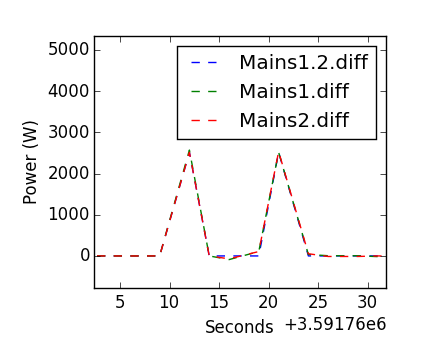
\includegraphics[width=0.5\textwidth]{multidisaggfig/heatingIndoorPhase12On.png} &
                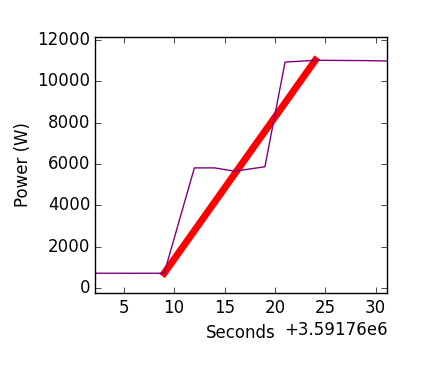
\includegraphics[width=0.5\textwidth]{multidisaggfig/heatingIndoorUp.png}\tabularnewline
                (a) & (b) \tabularnewline
                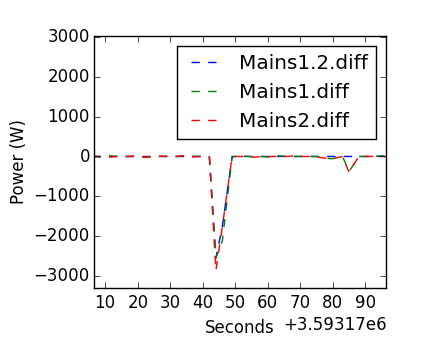
\includegraphics[width=0.5\textwidth]{multidisaggfig/heatingIndoorPhase12Off.png} &
                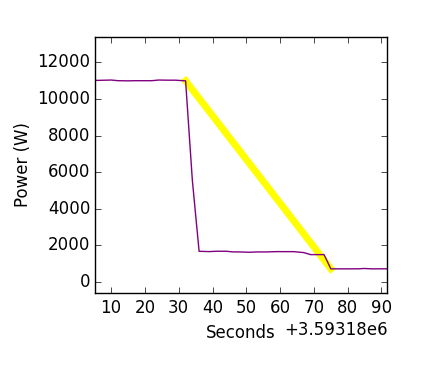
\includegraphics[width=0.5\textwidth]{multidisaggfig/heatingIndoorDown.png}\tabularnewline
                (c) & (d) \tabularnewline
                \end{tabular}
                }
        \caption{
        (a) On piecewise event and (c) Off piecewise event of heatingIndoor. heatingIndoor is disaggregated by motif mining the on event (b) and off event (d).}
        \label{fig_heatingIndoorResults}
\end{figure*}

Figure \ref{fig_heatingIndoorResults} (a) gives an example of 
an on event in the two-phase Mains1 and Mains2. 
Mains1.diff denotes the diffs data from Mains1 and Mains2.diff represents 
the diffs data from Mains2. 
Mains1.2.diff shows as blue when Mains1 and Mains2 share the similar power changes. 
We can see that 
the power consumption of a specific device jumps twice in two phases simultaneously.
The first time, both phases jump 2572W. After nine seconds, 
the power of both phases increases  2520W. 
The sum of these four changes is 10184W. 
Compared with the power levels of all devices, 
we speculate that these power changes are caused 
by the device heatingIndoor. 
%By applying multivariate piecewise motif mining, 
%we match the power consumption with $11000W$ and 
%categorize this on event into heating indoor. 
Figure \ref{fig_heatingIndoorResults} (b) shares the same snippet of time series as Figure \ref{fig_heatingIndoorResults} (a). 
The red line indicates that the on event of heatingIndoor is recognized.    
\begin{figure*}[!t]
        \centering{
                \begin{tabular}{cccc}
                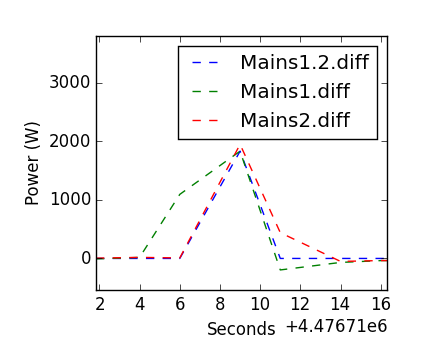
\includegraphics[width=0.5\textwidth]{multidisaggfig/dryerPhase12OnDiff.png} &
                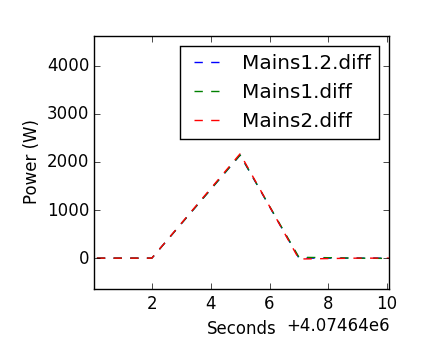
\includegraphics[width=0.5\textwidth]{multidisaggfig/waterHeaterPhase12OnDiff.png} \tabularnewline
                (a) & (b) \tabularnewline
                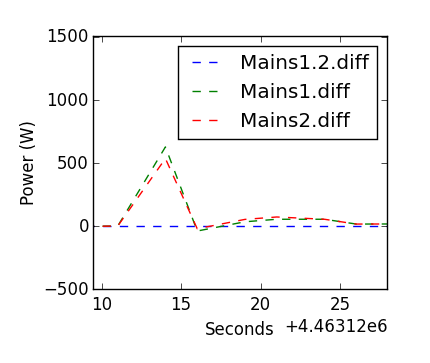
\includegraphics[width=0.5\textwidth]{multidisaggfig/heatingIndoorOutdoorPhase12On_1.png}&
                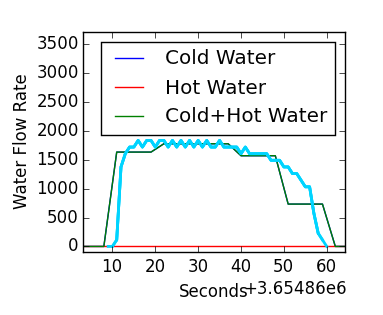
\includegraphics[width=0.5\textwidth]{multidisaggfig/UpToiletFitted.png}\tabularnewline
                (c) & (d) \tabularnewline
                \end{tabular}
                }
        \caption{
        Disaggregating dryer and continuous variable load heatingOutdoor with multivariate motif mining. The on event of a device and the corresponding diffs in the two phases for (a) dryer, (b) water heater, (c) heatingOutdoor. 
  	(d) Disaggregating the toilet water use end with dynamic time-warping subsequence search. This Y-axis is water flow rate in 10000*liter/minute.
        }
        \label{fig_dryerResults}
\end{figure*}

Similarly, the off event plunges twice in two seconds -2877W and -1759W in both phases, as shown in Figure \ref{fig_heatingIndoorResults} (c).
The sum of this off event is -9272W. 
After matching the power levels, we categorize it as the off event of heatingIndoor as indicated in Figure \ref{fig_heatingIndoorResults} (d). 

The dryer has the same power level as the waterheater at around 4800W. 
If we disaggregate these two devices from the sum of the two phases, 
it's difficult to distinguish them,  
but with multivariate piecewise motif mining, these two devices 
can be distinguished. 

%Figure \ref{fig_dryerResults} (a) and (b) shows the on event of dryer from sum of phase 1 and phase 2, 
%and these two phases separately. 
Figure \ref{fig_dryerResults} (a) and (b) are the diff data of the dryer and waterheater from the two-phase circuit. 
We can see that the waterheater draws power from Phase 1 and Phase 2 at the same time,  
but the dryer shows a different pattern. It draws power from Phase 1 at a lower power of 1093W, then jumps to 1830W; 
at the same time, it draws power from Phase 2 at the high level of 1946W immediately. 
We encode the power usage as shown in Figure \ref{fig_eventEncoding}, then apply motif mining to disaggregate them. 
 
After deleting the power consumption from both aggregated phases, 
we apply piecewise motif mining again to a single phase. 
We then discover the humidifier from Phase 1 
and the microwave from Phase 2. 
%Note that the power consumption of humidifier and microwave overlaps sometimes, 
%which makes it hard to separate them. 
%But they draw power from different phases separately. 
%Multivariate motif mining can separate them. 
When we only disaggregate the sum of Phase 1 and Phase 2, 
the precision recall result of the microwave and humidifier is not very accurate 
because sometimes their power consumptions are similar. 
However, using multivariate motif mining, we can separate them very clearly 
with good precision and recall. 
The precision and recall results for the data set Study10 are listed in Table \ref{table_study10results}.

Recursive multivariate motif mining is capable of disaggregating continuous variable loads. 
%\begin{figure*}[!t]
        \centering{
                \begin{tabular}{cccc}
                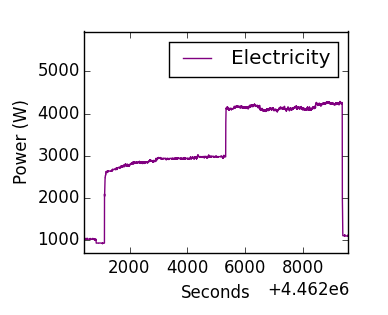
\includegraphics[width=3.2in]{multidisaggfig/heatingIndoorOutdoorPattern1_sum.png} &
                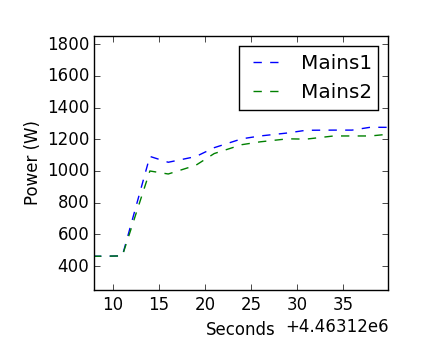
\includegraphics[width=3.2in]{multidisaggfig/heatingIndoorOutdoorPattern1.png} \tabularnewline
                 (a) & (b)\tabularnewline
                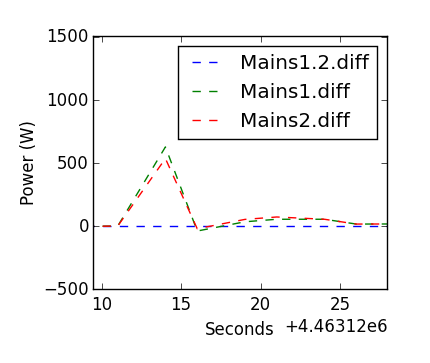
\includegraphics[width=3.2in]{multidisaggfig/heatingIndoorOutdoorPhase12On_1.png} &
                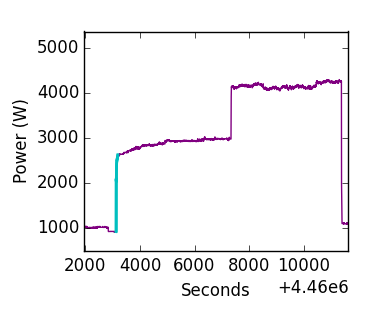
\includegraphics[width=3.2in]{multidisaggfig/heatingIndoorOutdoorFittedPattern1.png}\tabularnewline
                (c) &(d) \tabularnewline
                \end{tabular}
                }
        \caption{
        Disaggregating continuous variable load heating outdoor. 
        (a) the startup in the sum of aggregated power (b) the startup in two phases (c) the diffs in two phases (d) the disaggregated on event of heating outdoor.}
        \label{fig_heatingOutdoorResults}
\end{figure*}

Figure \ref{fig_dryerResults} (c) shows the diff data of heatingOutdoor from the two phases. 
During this on event, its power levels change nine times, then continue at a relatively stable state.
%Figure \ref{fig_heatingOutdoorResults} (a) illustrates the startup of heatingOutdoor.
%as shown in Figure \ref{fig_heatingOutdoorResults} (b) and (c). 
By applying piecewise motif mining, 
we can successfully identify this as the heatingOutdoor device 
after matching its power level. 
%The disaggregated result is displayed in Figure \ref{fig_dryerResults} (d).
%Note that this continuous variable load startup snippet can be discovered by dynamic time warping 
%subsequence search as well if this device is on without the intervene of other devices.
If another device  $D$ which draws from Phase 1 or Phase 2 is turned on or off during this period, 
multivariate piece-wise motif mining can still identify this heatingOutdoor device. 
This is because $D$ only uses one phase's power; 
hence its power change is not counted in our piecewise event. 

\iffalse
\subsubsection{Water Disaggregation and Constraints}
Water usage displays different characteristics. 
The total water consumption is zero most of the time.
Whenever a water use end is operated, water is consumed intensively for a period of time. 
Then it will stay off for a much longer time. 
We observe that the operations of water use ends reflect a series of user behaviors. 
For instance, a person may use the toilet in the bathroom first, 
then wash hands in the sink and finally take a shower afterwards. 
%This series of events highly affect electricity usage as well. 
%When the person enters into the bathroom, the light in the bathroom is turned on. 
%After using the bathroom, the person leaves and turns the light off. 
%Moreover, we observe that the usage of toilet is usually accompanied by
%sink usage afterwards. 

%In this subsection, we apply the semi-supervised multivariate piecewise motif mining 
%to water data. 
Similar to electricity disaggregation, we use a period of aggregated water usage 
data to extract features  
and obtain the water flow rate level of each water use end.
Table \ref{table_resultStudy10Water} lists the water consumption rate for each device. 
For instance, taking a shower uses hot water at a flow rate between 0.1822 liter/min and 0.1986 liter/min. 
Let $\frac{\alpha}{10000}$ denotes this range of water flow rate.
The total hot and cold water consumption by  shower is 0.1904 liter/min. 
Therefore, the cold water flow rate caused by shower is $0.1904-\frac{\alpha}{10000}$ liter/min. 
Turning on the water for the shower takes around two seconds. 
%The disaggregation results are shown in Table \ref{table_resultStudy10Water}.
%\begin{table*}[!t]
\renewcommand{\arraystretch}{1.3}
%\caption{Water Flow Rate Levels of Water End Uses and Disaggregation Results}
%\label{table_resultStudy10Water}
\tbl{Water Flow Rate Levels of Water End Uses and Disaggregation Results.\label{table_resultStudy10Water}}{
\centering
\begin{tabular}{|c|c|c|c|c|c|c|}
\hline
\multirow{2}{*}{Device} & \multirow{2}{*}{Hot water} & \multirow{2}{*}{Cold water} & \multirow{2}{*}{Duration} &  \multirow{2}{*}{Precision} & \multirow{2}{*}{Recall} &  \multirow{2}{*}{F-measure}\\
           &  (liter/min) & (l/min*10000)& (second) & & & \\
\hline
\hline
Shower & $\alpha \in (1822, 1986)$ & $1904-\alpha$& on: 2 & 0.999 & 0.972 & 0.986 \\
\hline
Washing Machine & $\alpha \in (1988, 2276)$  & $2132-\alpha$ & on: 5& 0.997  & 0.969 & 0.983\\
\hline
DownToilet & 0 & (1270, 1400) & whole: 50& NA & NA & NA\\
\hline
UpToilet & 0 & (1480, 1700) & whole: 50& NA & NA & NA \\
%\hline
%KitchenSink &  $ \alpha \in (0, 57) $ & 57- $\alpha$ & 2& & & \\
%\hline
%UpSink & 34 & 160 & 2& & & \\
%\hline
%DownSink & 57  & 80 & 2& & & \\
%\hline
%Dish Washer & 34 & -11 & 2& & & \\
\hline
\end{tabular}
}
\end{table*}
\begin{table}[h]
\renewcommand{\arraystretch}{1.3}
%\caption{Water Flow Rate Levels of Water End Uses.}
%\label{table_resultStudy10Water}
\tbl{Water Flow Rate Levels of Water End Uses and Disaggregation Results.\label{table_resultStudy10Water}}{
\centering
\small
\setlength\tabcolsep{2pt}
\begin{tabular}{|c|c|c|c|c|c|c|}
\hline
\multirow{2}{*}{Device} & \multirow{2}{*}{Hot water} & \multirow{2}{*}{Cold water} & \multirow{2}{*}{Duration}  \\
           &  (liter/min*10000) & (l/min*10000)  & (second)\\
\hline
\hline
Shower & $\alpha \in (1822, 1986)$ & $1904-\alpha$  & on: 2\\
\hline
Washing Machine & $\alpha \in (1988, 2276)$  & $2132-\alpha$ & on: 5\\
\hline
DownToilet & 0 & (1270, 1400) & whole: 50\\
\hline
UpToilet & 0 & (1480, 1700) & whole: 50\\
%\hline
%KitchenSink &  $ \alpha \in (0, 57) $ & 57- $\alpha$ & 2& & & \\
%\hline
%UpSink & 34 & 160 & 2& & & \\
%\hline
%DownSink & 57  & 80 & 2& & & \\
%\hline
%Dish Washer & 34 & -11 & 2& & & \\
\hline
\end{tabular}
}
\end{table}

After these calculations, we apply a multivariate piecewise motif mining approach to 
water disaggregation. 
For the shower and washing machine, 
the total flow rate of hot and cold water is high,  nearly 0.2 liter/minute. 
Therefore by only searching the 
total hot and cold water flow rate, we can identify these two devices. 
The event of shower usage usually lasts for more than one minute, 
but the washing machine uses water for less than one minute, 
repeating six to nine times. 
Both the shower and washing machine use 
hot water and cold water. 
However, the washing machine uses hot water for only the 
first one or two times. For the rest of its cycle, 
only cold water is used. 
Whenever the washing machines starts, 
the power consumption starts as well. 

%\begin{figure*}[!t]
        \centering{
                \begin{tabular}{cc}
                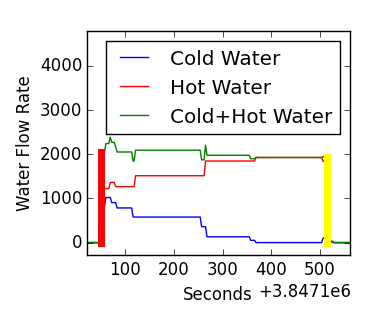
\includegraphics[width=0.5\textwidth]{multidisaggfig/showerFitted.png}&
                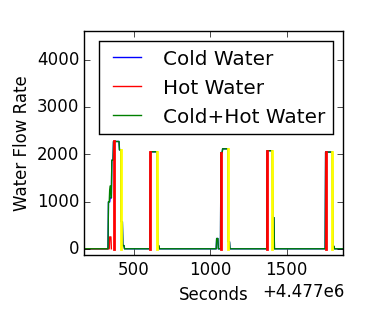
\includegraphics[width=0.5\textwidth]{multidisaggfig/washingMachineWaterFitted.png}\tabularnewline
                (a) & (b)\tabularnewline
                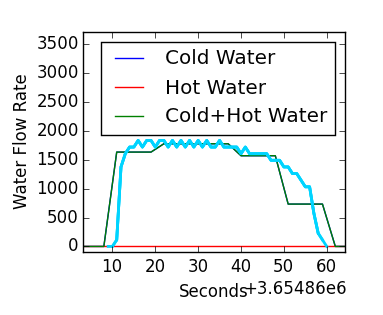
\includegraphics[width=0.5\textwidth]{multidisaggfig/UpToiletFitted.png}&
                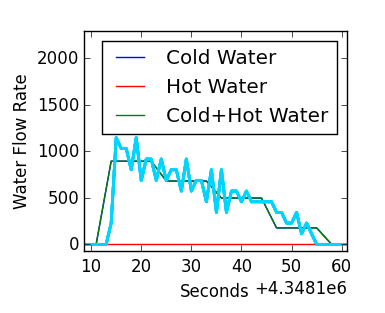
\includegraphics[width=0.5\textwidth]{multidisaggfig/DownToiletFitted.png}
                \tabularnewline
                 (c) & (d)\tabularnewline
                \end{tabular}
                }
        \caption{
        X-axis is the duration to a specific time in seconds, Y-axis is water flow rate in 10000*liter/minute. 
	(a) and (b) denote the water disaggregation of shower and washing machine. The fitted red line denotes the on event of water, and the fitted yellow line denotes the off event of water. 
	(c) and (d) are the disaggregated two toilets of complete usage cycle by dynamic time warping subsequence search. 
	}
        \label{fig_waterDisaggResults}
\end{figure*}
%Figure \ref{fig_waterDisaggResults} (a) and (b) display the water usage of shower and washing machine. 
Applying piecewise motif mining to the water usage lets us disaggregate the
shower and washing machine. %as in Figure \ref{fig_waterDisaggResults} (a) and (b).
The precision, recall and F-measure for the shower disaggregation are 
0.999, 0.972, and 0.986,  
and the precision, recall and F-measure for the washing machine disaggregation are 
0.997, 0.969, and 0.983. 
However, with a variable water flow rate, 
piecewise motif mining has limitations in handling water use ends such as the toilet.
Therefore we use the dynamic time warping subsequence~\cite{rakthanmanon2012searching} search as a complementary to discover these water use ends.  
For the two toilets, we apply dynamic time warping to match the time series.
The water usage results of one toilet, UpToilet, is shown in Figure \ref{fig_dryerResults} (d). 

%There are totally three sinks in the house, namely up sink, down sink and kitchen sink. 
%People may use sinks with only hot water or cold water, or both hot and cold water. 
%The water usage may be large or small. 
%In this case, it is hard to distinguish these three sinks. 
%However, by observing the water usage of up sink and down sink. 
%We find that there's correlation between the down sink and the down toilet, 
%up sink and up toilet. 
%Figure \ref{fig_ToiletSinkCorrelation} (a) and (b) show that the toilet and sink start almost at the same time, 
%or end at the same time. 
We can see that multivariate piecewise motif mining is capable of 
disaggregating water use ends which have sharp on/off water flow rates. 
However, it has limitations in dealing with water use ends with irregular water use patterns, 
such as toilets and sinks. 
Since the water usage of toilets is relatively fixed if used alone, 
some toilet water usages can be disaggregated by using the dynamic time warping subsequence search 
which was researched in \cite{nguyen2013development}. 
\fi
